% =====================================================================
%  Power-to-X (PtX) | Model answers to Examination Subjects A, B and C
%  Abdou Moumouni University, IMP-EGH | Prepared by KOUAME Koffi Fidele
%  Compile: pdflatex ptx_model_answers.tex (twice)
% =====================================================================
\documentclass[11pt,a4paper]{article}

\usepackage[T1]{fontenc}
\usepackage[utf8]{inputenc}
\usepackage{tgtermes}
\usepackage{mathptmx}
\usepackage[english]{babel}
\usepackage[a4paper,top=2.2cm,bottom=2.2cm,left=2.2cm,right=2.2cm,headsep=0.6cm]{geometry}
\usepackage{microtype}
\usepackage{amsmath,amssymb}
\usepackage[table]{xcolor}
\usepackage{graphicx}
\usepackage{tabularx,array,booktabs,multirow}
\usepackage{enumitem}
\usepackage{titlesec}
\usepackage{fancyhdr}
\usepackage[most]{tcolorbox}
\usepackage[hidelinks]{hyperref}
\usepackage{xurl}
\usepackage{caption}
\usepackage{needspace}
\urlstyle{same}

% ---- colours (matching the subject sheets)
\definecolor{uamred}{HTML}{C00000}
\definecolor{egh}{HTML}{6AA84F}
\definecolor{rulegray}{HTML}{A59F93}
\definecolor{boxgray}{HTML}{E6E6E6}
\definecolor{ans}{HTML}{1E6B32}
\definecolor{navy}{HTML}{1F3A5F}

% ---- layout
\setlength{\parindent}{0pt}
\setlength{\parskip}{4pt}
\setlist{nosep,itemsep=2pt,leftmargin=1.4em}
\captionsetup{font=small,labelfont=bf}

\titleformat{\section}{\Large\bfseries}{}{0pt}{}
\titlespacing*{\section}{0pt}{12pt}{6pt}
\titleformat{\subsection}{\large\bfseries}{}{0pt}{}
\titlespacing*{\subsection}{0pt}{9pt}{4pt}

\pagestyle{fancy}
\fancyhf{}
\fancyhead[L]{\small\textbf{Power-to-X (PtX) | Model answers}}
\fancyhead[R]{\small IMP-EGH | System Analysis | 2026}
\fancyfoot[C]{\small\thepage}
\renewcommand{\headrulewidth}{0.6pt}

% ---- answer macros
\newcolumntype{Y}{>{\raggedright\arraybackslash}X}
\newcommand{\degC}{\,\textdegree C}
\newcommand{\q}[2]{\par\medskip\textbf{#1.} #2\par}
\newcommand{\answer}[2]{\textcolor{ans}{\textbf{Answer #1}}, #2\par}
\newcommand{\why}[1]{\textit{Justification.} #1\par}
\newcommand{\fillin}[1]{\textcolor{ans}{\textbf{#1}}}
\newcommand{\pts}[1]{\hfill{\normalsize\textbf{(#1)}}}
\newcommand{\rxn}[1]{\[\mathrm{#1}\]}

\newtcolorbox{keybox}[1]{colback=boxgray!40,colframe=black,boxrule=0pt,leftrule=2.5pt,
  arc=0pt,left=6pt,right=6pt,top=3pt,bottom=4pt,
  title={\textbf{#1}},coltitle=black,colbacktitle=boxgray,attach title to upper={\par\smallskip}}

\begin{document}

% =====================================================================
%  COVER PAGE
% =====================================================================
\begin{titlepage}
\thispagestyle{empty}
\begin{minipage}[c]{0.2\textwidth}
  
\includegraphics[width=\linewidth]{logo_uam.png}
\end{minipage}%
\begin{minipage}[c]{0.58\textwidth}
  \centering
  {\Large\bfseries\textcolor{uamred}{A}bdou \textcolor{uamred}{M}oumouni \textcolor{uamred}{U}niversity}\\[6pt]
  {\small\bfseries\textcolor{egh}{I}nternational \textcolor{egh}{M}aster \textcolor{egh}{P}rogram in
   \textcolor{egh}{E}nergy and \textcolor{egh}{G}reen \textcolor{egh}{H}ydrogen}\\[4pt]
  {\bfseries (IMP-EGH)}
\end{minipage}%
\begin{minipage}[c]{0.22\textwidth}
  \raggedleft
\includegraphics[width=0.95\linewidth]{logo_impegh.png}
\end{minipage}

\vspace{10pt}
{\color{rulegray}\rule{\textwidth}{2.2pt}}

\vspace*{5.2cm}
\begin{center}
{\fontsize{30}{36}\selectfont\bfseries Model Answers}\\[12pt]
{\Large\itshape Power-to-X (PtX)}\\[8pt]
{\large Part 1: Foundations\quad Part 2: Pathways\quad Case-study projects}\\[24pt]
{\large Worked solutions to the three 1-hour subjects (A, B, C)}\\[2pt]
{\large with justifications, calculations and the Kassø e-Methanol case study}
\end{center}

\vfill
\begin{minipage}[t]{0.5\textwidth}
\textbf{Course lecturer}\\[3pt]
Dr Bachir Yaou Balarabe\\
Islamic University of Niger
\end{minipage}%
\begin{minipage}[t]{0.5\textwidth}
\raggedleft
\textbf{Prepared by}\\[3pt]
KOUAME Koffi Fidèle\\
IMP-EGH, option System Analysis
\end{minipage}

\vspace{2.2cm}
\begin{center}\textbf{October 2026}\end{center}
\end{titlepage}

% =====================================================================
%  ANSWER KEY
% =====================================================================
\begin{center}
{\LARGE\bfseries Answer Key at a Glance}\\[3pt]
{\large Power-to-X (PtX)}
\end{center}

\begin{keybox}{How to use this document}
\begin{itemize}
  \item The key below lists the expected answers to Parts A and B of each subject (T = True, F = False).
  \item The following sections give, for every question, the answer and a short justification taken from
        the course, followed by the completed tables (Part C), the balanced reactions with conditions
        (Part D) and a full answer to the case study (Part E) for Project 4, Kassø e-Methanol.
  \item Values written as ranges are typical values from the course and the literature; figures on the Kassø
        plant come from the developer's public communications (see References).
\end{itemize}
\end{keybox}

\medskip
\textbf{Part A. Multiple-choice questions}\par
\smallskip
{\centering
\renewcommand{\arraystretch}{1.3}
\begin{tabular}{l*{8}{c}}
\toprule
\textbf{Subject} & \textbf{A1} & \textbf{A2} & \textbf{A3} & \textbf{A4} & \textbf{A5} & \textbf{A6} & \textbf{A7} & \textbf{A8}\\
\midrule
A & B & D & A & D & B & C & B & D\\
B & B & A & B & D & B & B & A & B\\
C & D & C & B & A & D & B & A & A\\
\bottomrule
\end{tabular}\par}

\medskip
\textbf{Part B. True or False}\par
\smallskip
{\centering
\renewcommand{\arraystretch}{1.3}
\begin{tabular}{l*{8}{c}}
\toprule
\textbf{Subject} & \textbf{B1} & \textbf{B2} & \textbf{B3} & \textbf{B4} & \textbf{B5} & \textbf{B6} & \textbf{B7} & \textbf{B8}\\
\midrule
A & T & T & F & F & F & T & F & T\\
B & T & F & F & T & T & F & T & F\\
C & T & F & T & F & T & T & F & T\\
\bottomrule
\end{tabular}\par}

\medskip
\begin{keybox}{Key figures used in the answers}
\begin{itemize}
  \item Molar masses: CH$_3$OH 32.04, H$_2$ 2.016, CO$_2$ 44.01, H$_2$O 18.015 g/mol.
  \item Stoichiometry of methanol from CO$_2$: per tonne of CH$_3$OH, 0.189 t H$_2$, 1.374 t CO$_2$
        and 0.562 t H$_2$O by-product.
  \item Theoretical water need of electrolysis: 18.015/2.016 = 8.94 kg H$_2$O per kg H$_2$.
  \item Kassø plant: 42,000 t/yr e-methanol, three PEM electrolysers of about 52 MW in total (Siemens Energy),
        304 MW solar park supplying about half of the electricity, biogenic CO$_2$, RFNBO-certified (2025).
\end{itemize}
\end{keybox}

% =====================================================================
%  SUBJECT A
% =====================================================================
\clearpage
\begin{center}
{\LARGE\bfseries Model Answers | Subject A}\\[3pt]
{\large Power-to-X (PtX)}
\end{center}

\section{Part A. Multiple-choice questions \pts{8 $\times$ 0.5 = 4 pts}}

\q{A1}{In ``Power-to-X'', the letter X designates:}
\answer{B}{the final product (carrier, fuel, chemical or heat).}
\why{``Power'' is the renewable electricity input; ``X'' is the output: hydrogen or a hydrogen-derived carrier
(ammonia, methanol, synthetic methane, liquid fuels), a chemical, or heat.}

\q{A2}{In a PEM electrolyser, the reaction at the anode is:}
\answer{D}{$\mathrm{H_2O \longrightarrow \tfrac{1}{2}O_2 + 2\,H^+ + 2\,e^-}$.}
\why{The PEM electrolyte is acidic and conducts protons. Water is oxidised at the anode (oxygen evolution);
the protons cross the membrane and are reduced at the cathode ($\mathrm{2\,H^+ + 2\,e^- \rightarrow H_2}$).
Option A is the SOEC anode, option C the alkaline cathode, option B a cathode reaction.}

\q{A3}{The electrolyte of a solid oxide electrolyser (SOEC) is typically:}
\answer{A}{yttria-stabilised zirconia (YSZ).}
\why{YSZ is a ceramic that conducts O$^{2-}$ ions at 600--1000\degC. Nafion is the PEM membrane, 25--30\,\% KOH
the alkaline electrolyte, and molten carbonate the MCFC electrolyte.}

\q{A4}{Catalyst and pressure of green methanol synthesis:}
\answer{D}{Cu/ZnO-based catalyst, 50--100 bar.}
\why{Methanol synthesis uses Cu/ZnO/Al$_2$O$_3$ at about 200--300\degC{} and 50--100 bar. An iron catalyst at
150--300 bar describes Haber--Bosch; Co or Fe at low pressure describes Fischer--Tropsch.}

\q{A5}{Reaction that prepares syngas for Fischer--Tropsch from green H$_2$ and captured CO$_2$:}
\answer{B}{$\mathrm{H_2 + CO_2 \longrightarrow CO + H_2O}$, the reverse water-gas shift (RWGS).}
\why{FT synthesis needs CO, not CO$_2$. The endothermic RWGS ($\Delta H \approx +41$ kJ/mol) converts captured
CO$_2$ into CO, which is then mixed with H$_2$ to reach H$_2$/CO $\approx 2$.}

\q{A6}{A fuel cell with a molten lithium/potassium carbonate electrolyte operates at about:}
\answer{C}{650\degC.}
\why{The MCFC electrolyte must be molten to conduct CO$_3^{2-}$ ions, which requires about 600--700\degC.}

\q{A7}{Overall power-to-methanol/DME efficiency given in the course:}
\answer{B}{50--55\,\%.}
\why{Electrolysis (60--70\,\% LHV) is followed by synthesis and distillation losses. Check: 0.189 t H$_2$ per tonne
of methanol at about 55 kWh/kg gives 10.4 MWh, against 5.5 MWh of methanol (LHV 19.9 GJ/t), that is about
53\,\%.}

\q{A8}{For a plant driven mainly by a solar park, like Kassø, the best-suited electrolyser is:}
\answer{D}{PEM, because of its response in seconds and wide partial-load range.}
\why{Solar output varies within minutes and falls to zero at night. PEM follows these variations; AWE has a
minimum load of 15--40\,\% and slower dynamics, and SOEC needs a steady high-grade heat source.}

\section{Part B. True or False \pts{8 $\times$ 0.5 = 4 pts}}

{\small
\renewcommand{\arraystretch}{1.35}
\begin{tabularx}{\linewidth}{@{}p{0.6cm}>{\raggedright\arraybackslash}p{5.6cm}c>{\raggedright\arraybackslash}X@{}}
\toprule
\textbf{No.} & \textbf{Statement} & \textbf{T/F} & \textbf{Correction or justification}\\
\midrule
B1 & Electrolytic hydrogen routinely reaches 99.99\,\% purity. & \fillin{T} &
  Electrolysis gives very pure H$_2$ (99.9 to 99.999\,\% after drying and deoxidation), suitable for fuel cells. \\
B2 & Direct air capture extracts CO$_2$ from ambient air at about 420 ppm. & \fillin{T} &
  The very low concentration is why DAC is the most energy-intensive and costly CO$_2$ source. \\
B3 & Alkaline electrolysers need platinum-group metal catalysts. & \fillin{F} &
  \textbf{Correction:} AWE uses non-noble nickel-based electrodes; PEM needs platinum (cathode) and iridium (anode). \\
B4 & Methanation $\mathrm{CO_2 + 4\,H_2 \rightarrow CH_4 + 2\,H_2O}$ is endothermic. & \fillin{F} &
  \textbf{Correction:} it is strongly exothermic, $\Delta H^\circ_{298} = -165$ kJ/mol; heat must be removed. \\
B5 & In an alkaline fuel cell (AFC), water is produced at the cathode. & \fillin{F} &
  \textbf{Correction:} water is produced at the anode: $\mathrm{H_2 + 2\,OH^- \rightarrow 2\,H_2O + 2\,e^-}$. \\
B6 & Biogenic CO$_2$ supply may be more dispersed and seasonal than industrial point sources. & \fillin{T} &
  Biogas and bioethanol plants are small, scattered and depend on feedstock seasons, unlike cement or steel plants. \\
B7 & The round-trip efficiency of Power-to-Power (30--45\,\%) is higher than that of batteries. & \fillin{F} &
  \textbf{Correction:} it is lower; batteries reach about 80--95\,\%. Power-to-Power is justified for long-duration and seasonal storage. \\
B8 & Without heat recovery, power-to-SNG efficiency is 50--65\,\%; with heat recovery it can exceed 70--80\,\%. & \fillin{T} &
  Recovering the methanation and electrolyser heat (district heating, process heat) raises the useful-energy efficiency. \\
\bottomrule
\end{tabularx}}

\section{Part C. Complete the missing information \pts{3 pts}}

\textbf{Electrolyser technology comparison matrix} (answers in green).

{\small
\renewcommand{\arraystretch}{1.35}
\begin{tabularx}{\linewidth}{@{}>{\raggedright\arraybackslash}p{3.2cm}YYYY@{}}
\toprule
\textbf{Factor} & \textbf{Alkaline (ALK)} & \textbf{PEM} & \textbf{AEM} & \textbf{SOEC}\\
\midrule
Electrolyte & \fillin{Aqueous KOH (25--30\,\%)} & Solid polymer & Solid anion membrane & \fillin{Ceramic YSZ (O$^{2-}$ conductor)}\\
Operating temperature & 60--90\degC & \fillin{50--80\degC} & 40--70\degC & 600--1000\degC\\
Response time & Slow & Fast & \fillin{Fast} & Slow\\
Maturity & \fillin{Mature (commercial for decades)} & Commercialized & Emerging & Pre-commercial\\
Lifetime (h) & 60,000--90,000 & 30,000--90,000 & 10,000--20,000 & \fillin{$<$ 20,000 (about 10,000--20,000)}\\
\bottomrule
\end{tabularx}}

\section{Part D. Reactions \pts{3 pts}}

\needspace{6\baselineskip}\textbf{D1. Complete and name $\mathrm{CO_2 + 4\,H_2 \longrightarrow \dots}$} \pts{0.75 pt}
\rxn{CO_2 + 4\,H_2 \longrightarrow CH_4 + 2\,H_2O \qquad \Delta H^\circ_{298} = -165\ kJ/mol}
Sabatier reaction (catalytic CO$_2$ methanation), the core of Power-to-Methane. Nickel-based catalyst
(ruthenium as an alternative), about 250--400\degC{} and 1--30 bar. The reaction is exothermic and reduces the number
of gas moles (5 to 3), so it is favoured by moderate temperature and higher pressure.

\needspace{6\baselineskip}\textbf{D2. Methanol to dimethyl ether (DME) and type of reaction} \pts{0.75 pt}
\rxn{2\,CH_3OH \longrightarrow CH_3OCH_3 + H_2O \qquad \Delta H \approx -23.4\ kJ/mol}
Catalytic dehydration (condensation) of methanol over a solid acid catalyst ($\gamma$-Al$_2$O$_3$ or zeolite),
about 250--400\degC{} and 10--20 bar. It is mildly exothermic.

\needspace{6\baselineskip}\textbf{D3. Half-reactions and overall reaction of a PEM fuel cell} \pts{0.75 pt}
\begin{align*}
\text{Anode (oxidation):}\quad & \mathrm{H_2 \longrightarrow 2\,H^+ + 2\,e^-}\\
\text{Cathode (reduction):}\quad & \mathrm{\tfrac{1}{2}O_2 + 2\,H^+ + 2\,e^- \longrightarrow H_2O}\\
\text{Overall:}\quad & \mathrm{H_2 + \tfrac{1}{2}O_2 \longrightarrow H_2O} \qquad E^\circ = 1.23\ \mathrm{V},\ \Delta G^\circ = -237\ \mathrm{kJ/mol}
\end{align*}
Protons cross the polymer membrane; water forms at the cathode; operation at about 60--80\degC.

\needspace{6\baselineskip}\textbf{D4. Kassø synthesis reaction and reactant masses per tonne of methanol} \pts{0.75 pt}
\rxn{CO_2 + 3\,H_2 \longrightarrow CH_3OH + H_2O \qquad \Delta H^\circ_{298} \approx -49.5\ kJ/mol}
Cu/ZnO/Al$_2$O$_3$ catalyst, about 200--300\degC{} and 50--100 bar.
\begin{align*}
n(\mathrm{CH_3OH}) &= \frac{10^6\ \mathrm{g}}{32.04\ \mathrm{g/mol}} = 31{,}211\ \mathrm{mol}\\
m(\mathrm{H_2}) &= 3 \times 31{,}211 \times 2.016 = 188{,}800\ \mathrm{g} \approx \mathbf{0.189\ t}\\
m(\mathrm{CO_2}) &= 31{,}211 \times 44.01 = 1{,}373{,}600\ \mathrm{g} \approx \mathbf{1.374\ t}
\end{align*}
Each tonne of methanol therefore needs about 189 kg of H$_2$ and 1.37 t of CO$_2$, and releases 0.56 t of water.
In practice the consumption is slightly higher because of purge losses and side products.

\section{Part E. Case study: Project 4, Kassø e-Methanol (Denmark) \pts{6 pts}}

\needspace{6\baselineskip}\textbf{E1. Name, country, developers or owners and main objective} \pts{1 pt}
\begin{itemize}
  \item \textbf{Name and location:} Kassø e-methanol facility (Kassø Power-to-X), Kassø, near Aabenraa, Southern
        Jutland, Denmark.
  \item \textbf{Developer and owners:} developed by the Danish renewable-energy company European Energy, owned
        51\,\% by European Energy and 49\,\% by Mitsui \& Co. (Japan). Electrolysers supplied by Siemens Energy;
        methanol loop designed and built by European Energy.
  \item \textbf{Milestones:} first green hydrogen in January 2025, first e-methanol in March 2025, RFNBO
        certification (ISCC EU) in April 2025, official inauguration on 13 May 2025.
  \item \textbf{Main objective:} produce up to 42,000 t/yr of e-methanol at the world's first commercial-scale
        e-methanol plant, to decarbonise shipping (A.P. Moller-Maersk) and chemical and plastic production
        (LEGO Group, Novo Nordisk; OMV as additional offtaker), and to demonstrate Power-to-X at industrial scale.
\end{itemize}

\needspace{6\baselineskip}\textbf{E2. Power-to-X pathway as a chain of steps and core reaction} \pts{1.5 pts}

\begin{figure}[h]
\centering
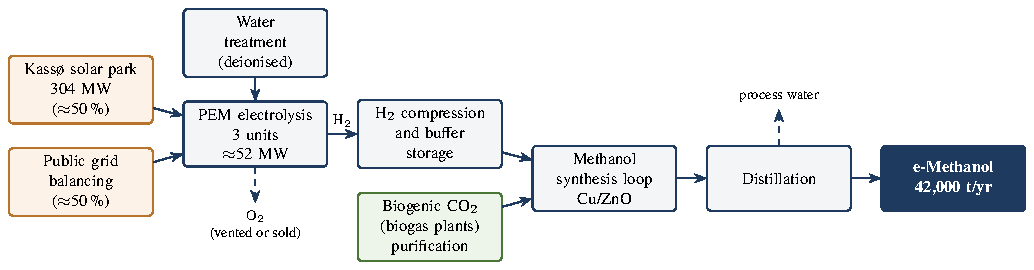
\includegraphics[width=\linewidth]{flow_kasso.pdf}
\caption{Simplified process chain of the Kassø e-methanol plant (dashed arrows: by-products).}
\end{figure}

\begin{enumerate}
  \item Renewable electricity: 304 MW Kassø solar park (about 50\,\%) and grid electricity under a balancing
        agreement (about 50\,\%).
  \item Water treatment to deionised quality, then PEM electrolysis (three units, about 52 MW):
        $\mathrm{2\,H_2O \rightarrow 2\,H_2 + O_2}$.
  \item Hydrogen compression and buffer storage, which decouples variable electrolysis from the synthesis loop.
  \item Biogenic CO$_2$ captured at biogas plants (the first batch came from Tønder), purified and delivered.
  \item Catalytic methanol synthesis in a recycle loop, then distillation to remove water.
  \item Storage and delivery of e-methanol to offtakers.
\end{enumerate}
Core reaction: $\mathrm{CO_2 + 3\,H_2 \rightarrow CH_3OH + H_2O}$ ($\Delta H \approx -49.5$ kJ/mol). Combined with
electrolysis, the net Power-to-Methanol balance is $\mathrm{CO_2 + 2\,H_2O \rightarrow CH_3OH + \tfrac{3}{2}O_2}$.

\needspace{6\baselineskip}\textbf{E3. Key technical data and choice of electrolyser} \pts{1.5 pts}

{\small
\renewcommand{\arraystretch}{1.3}
\begin{tabularx}{\linewidth}{@{}>{\raggedright\arraybackslash}p{3.6cm}X@{}}
\toprule
\textbf{Item} & \textbf{Value}\\
\midrule
Capacity & 42,000 t/yr e-methanol (about 53 million litres)\\
Electrolysis & PEM, Siemens Energy, three units, about 52 MW in total\\
Hydrogen & about 6,000 t/yr (project page) to 8,000 t/yr (2025 media kit); stoichiometry for 42,000 t requires 7,930 t\\
Power supply & 304 MW solar park (about 50\,\%) and grid (about 50\,\%)\\
Carbon source & Biogenic CO$_2$ from biogas plants, about 57,700 t/yr at nameplate\\
Product quality & Industry-grade e-methanol, certified RFNBO under the EU scheme ISCC EU\\
\bottomrule
\end{tabularx}}

\medskip
\textbf{Why PEM.} The plant is driven by solar power, which varies within minutes and stops at night. PEM electrolysers
respond in seconds, operate over a wide partial-load range, start quickly, deliver high-purity hydrogen at elevated
pressure and are compact. Alkaline electrolysers are cheaper but have a minimum load of 15--40\,\% and slower dynamics;
SOEC requires a steady high-temperature heat source that a solar-driven site does not have. The cost of PEM (platinum
and iridium catalysts, ultrapure water) is accepted in exchange for flexibility.

\needspace{6\baselineskip}\textbf{E4. Improvement question: which inputs would you change?} \pts{2 pts}

The plant has four inputs: electricity, water, CO$_2$ and heat. In order of impact:
\begin{enumerate}
  \item \textbf{Electricity.} Hybridise the supply with dedicated wind power purchase agreements. Danish solar has a
        capacity factor of only about 11--12\,\%, while wind reaches 30--45\,\%; a hybrid profile raises electrolyser
        full-load hours, lowers the cost per kilogram of hydrogen and secures hourly renewable matching, which EU
        RFNBO rules require from 2030.
  \item \textbf{Heat.} Recover electrolyser waste heat (30--40\,\% of the input, at 50--80\degC) and the exothermic
        synthesis heat for distillation and district heating. This raises the useful-energy efficiency well above the
        50--55\,\% of the methanol product alone.
  \item \textbf{Water.} Recycle the 0.56 t of process water released per tonne of methanol to the electrolysers.
        At nameplate this is about 23,600 t/yr, roughly one third of the theoretical demand of about 71,000 t/yr.
  \item \textbf{CO$_2$.} Contract several biogenic sources and add liquid CO$_2$ storage, since biogenic supply is
        dispersed and seasonal; direct air capture can be a long-term complement.
  \item \textbf{By-product oxygen.} Sell the oxygen (about 8 kg per kg H$_2$, around 60,000 t/yr) to wastewater,
        medical or industrial users to add revenue.
\end{enumerate}

\begin{center}\textit{End of Subject A}\end{center}

% =====================================================================
%  SUBJECT B
% =====================================================================
\clearpage
\begin{center}
{\LARGE\bfseries Model Answers | Subject B}\\[3pt]
{\large Power-to-X (PtX)}
\end{center}

\section{Part A. Multiple-choice questions \pts{8 $\times$ 0.5 = 4 pts}}

\q{A1}{The first documented Power-to-X projects appeared around:}
\answer{B}{1990.}
\why{Reviews of demonstration projects list the first plants from the late 1980s and early 1990s (for example
Higashi-Hiroshima 1988, Fayetteville 1991, PHOEBUS in Jülich 1993). 1839 is Grove's fuel cell, not a PtX project.}

\q{A2}{In an AWE, the electrolyte is typically:}
\answer{A}{25--30\,\% aqueous KOH.}
\why{Alkaline electrolysers use a concentrated potassium hydroxide solution and nickel electrodes; OH$^-$ is the
charge carrier.}

\q{A3}{Theoretical water consumption of electrolysis:}
\answer{B}{9 kg H$_2$O per kg H$_2$.}
\why{From $\mathrm{H_2O \rightarrow H_2 + \tfrac{1}{2}O_2}$: $18.015/2.016 = 8.94$ kg of water per kg of hydrogen.
Real plants need about 10--15 kg because of water treatment losses.}

\q{A4}{Typical operating conditions of Haber--Bosch synthesis:}
\answer{D}{150--300 bar, 400--500\degC, iron-based catalyst.}
\why{High pressure shifts the equilibrium towards ammonia (4 moles of gas give 2); 400--500\degC{} gives acceptable
kinetics on the promoted iron catalyst. Option B describes methanol synthesis.}

\q{A5}{CO$_2$ source with a high concentration (10--30\,\% or more):}
\answer{B}{industrial point sources (cement, steel, refineries).}
\why{The higher the CO$_2$ concentration, the lower the capture energy and cost. Air contains only about 420 ppm.}

\q{A6}{To stay competitive without heavy subsidies, renewable electricity should ideally cost less than:}
\answer{B}{30--40 \texteuro/MWh.}
\why{Electricity is the largest cost item of green hydrogen: at about 55 kWh/kg, each 10 \texteuro/MWh adds about
0.55 \texteuro/kg H$_2$.}

\q{A7}{Why is intermediate H$_2$ storage recommended between electrolysers and synthesis units?}
\answer{A}{to buffer slower synthesis units while fast electrolysers track variable renewable surplus.}
\why{Synthesis loops (methanol, ammonia, methanation) prefer steady operation and ramp slowly, whereas the
electrolyser follows the renewable profile; the buffer decouples the two.}

\q{A8}{Share of global anthropogenic CO$_2$ from conventional ammonia production:}
\answer{B}{1.2\,\%.}
\why{Conventional ammonia relies on steam methane reforming or coal gasification and accounts for roughly 1--2\,\%
of global CO$_2$ emissions.}

\section{Part B. True or False \pts{8 $\times$ 0.5 = 4 pts}}

{\small
\renewcommand{\arraystretch}{1.35}
\begin{tabularx}{\linewidth}{@{}p{0.6cm}>{\raggedright\arraybackslash}p{5.6cm}c>{\raggedright\arraybackslash}X@{}}
\toprule
\textbf{No.} & \textbf{Statement} & \textbf{T/F} & \textbf{Correction or justification}\\
\midrule
B1 & More than 80\,\% of current final energy still comes from fossil fuels. & \fillin{T} &
  Fossil fuels still supply about four fifths of global energy, which motivates Power-to-X for hard-to-electrify uses. \\
B2 & Power-to-Heat is a hydrogen-based PtX route treated in detail in the series. & \fillin{F} &
  \textbf{Correction:} Power-to-Heat converts electricity directly into heat without hydrogen; the series focuses on hydrogen-based routes. \\
B3 & AWE has a faster dynamic response than PEM. & \fillin{F} &
  \textbf{Correction:} PEM is faster (seconds); AWE is slower and has a minimum load of 15--40\,\%. \\
B4 & Ammonia combustion or cracking produces no CO$_2$, only N$_2$ and water (NO$_x$ must be controlled). & \fillin{T} &
  NH$_3$ contains no carbon: $\mathrm{4\,NH_3 + 3\,O_2 \rightarrow 2\,N_2 + 6\,H_2O}$. \\
B5 & In a PAFC, water is produced at the cathode and the cell tolerates CO$_2$ in air. & \fillin{T} &
  The acid electrolyte conducts H$^+$ to the cathode, and unlike the alkaline AFC it does not react with CO$_2$. \\
B6 & Biological methanation needs 200--400\degC{} and 30 bar. & \fillin{F} &
  \textbf{Correction:} biological methanation uses archaea at about 30--70\degC{} and near-ambient to moderate pressure (1--10 bar); 200--400\degC{} applies to catalytic methanation. \\
B7 & Additionality means the renewable generation used must be new, not diverted from other consumers. & \fillin{T} &
  This is the EU RFNBO additionality principle (Delegated Regulation 2023/1184). \\
B8 & Electrolyser flexibility always increases utilisation and therefore always lowers costs. & \fillin{F} &
  \textbf{Correction:} following variable power often lowers full-load hours and raises capital cost per kg; flexibility lowers cost only when the savings on electricity exceed this effect. \\
\bottomrule
\end{tabularx}}

\section{Part C. Complete the missing information \pts{3 pts}}

\textbf{Fuel-cell types} (answers in green).

{\small
\renewcommand{\arraystretch}{1.35}
\begin{tabularx}{\linewidth}{@{}lYYYY@{}}
\toprule
\textbf{Type} & \textbf{Electrolyte} & \textbf{Mobile ion} & \textbf{Temperature} & \textbf{Water produced at}\\
\midrule
AFC & Aqueous KOH & \fillin{OH$^-$} & $\sim$60--90\degC & \fillin{anode}\\
PAFC & \fillin{Liquid phosphoric acid (H$_3$PO$_4$)} & H$^+$ & $\sim$150--200\degC & cathode\\
PEMFC & Solid polymer membrane & H$^+$ & \fillin{$\sim$60--80\degC} & cathode\\
MCFC & Molten Li/K carbonate & \fillin{CO$_3^{2-}$} & $\sim$650\degC & anode\\
SOFC & Solid ceramic (zirconia) & O$^{2-}$ & $\sim$800--1000\degC & \fillin{anode}\\
\bottomrule
\end{tabularx}}

\section{Part D. Reactions \pts{3 pts}}

\needspace{6\baselineskip}\textbf{D1. Overall water electrolysis and gas formed at the cathode} \pts{0.75 pt}
\rxn{2\,H_2O \longrightarrow 2\,H_2 + O_2 \qquad \Delta H^\circ = +286\ kJ/mol\ H_2\ (HHV)}
Reversible voltage 1.23 V, thermoneutral voltage 1.48 V. \textbf{Hydrogen forms at the cathode} (reduction) and oxygen
at the anode, in a 2:1 volume ratio.

\needspace{6\baselineskip}\textbf{D2. Half-reactions of alkaline water electrolysis} \pts{0.75 pt}
\begin{align*}
\text{Cathode:}\quad & \mathrm{2\,H_2O + 2\,e^- \longrightarrow H_2 + 2\,OH^-}\\
\text{Anode:}\quad & \mathrm{2\,OH^- \longrightarrow \tfrac{1}{2}O_2 + H_2O + 2\,e^-}\\
\text{Overall:}\quad & \mathrm{H_2O \longrightarrow H_2 + \tfrac{1}{2}O_2}
\end{align*}
OH$^-$ ions migrate through the diaphragm from the cathode to the anode, in 25--30\,\% KOH at 60--90\degC.

\needspace{6\baselineskip}\textbf{D3. Haber--Bosch reaction, conditions and catalyst} \pts{0.75 pt}
\rxn{N_2 + 3\,H_2 \rightleftharpoons 2\,NH_3 \qquad \Delta H^\circ = -92\ kJ/mol}
Promoted iron catalyst (magnetite with K$_2$O and Al$_2$O$_3$), 150--300 bar, 400--500\degC. Conversion per pass is
only about 15--25\,\%, so unreacted gas is recycled after ammonia condensation.

\needspace{6\baselineskip}\textbf{D4. Steam reforming and water-gas shift, and why they are not used at Kassø} \pts{0.75 pt}
\begin{align*}
\text{Steam methane reforming:}\quad & \mathrm{CH_4 + H_2O \longrightarrow CO + 3\,H_2} \qquad \Delta H^\circ = +206\ \mathrm{kJ/mol}\ (\text{Ni},\ 850\text{--}950\,^\circ\mathrm{C})\\
\text{Water-gas shift:}\quad & \mathrm{CO + H_2O \longrightarrow CO_2 + H_2} \qquad \Delta H^\circ = -41\ \mathrm{kJ/mol}
\end{align*}
These reactions make hydrogen and syngas from fossil methane and release about 9--10 kg of CO$_2$ per kg of H$_2$. At
Kassø, hydrogen comes from water electrolysis powered by renewable electricity, and carbon comes from biogenic CO$_2$
that is hydrogenated directly ($\mathrm{CO_2 + 3\,H_2 \rightarrow CH_3OH + H_2O}$). No fossil feedstock and no
reforming step are needed, which is the condition for RFNBO status.

\section{Part E. Case study: Project 4, Kassø e-Methanol (Denmark) \pts{6 pts}}

\needspace{6\baselineskip}\textbf{E1. Renewable energy sources and their proportion} \pts{1 pt}

About \textbf{50\,\%} of the electricity comes from the adjacent \textbf{304 MW Kassø solar park}, one of the
largest in Northern Europe. The other \textbf{50\,\%} comes from the \textbf{public grid} through a balancing
agreement (Danske Commodities); in Denmark this supply is dominated by wind power. The grid share compensates for
the low capacity factor of Danish solar (about 11--12\,\%) and keeps the electrolysers running outside sunny hours.

\needspace{6\baselineskip}\textbf{E2. Environmental benefits and EU condition} \pts{1 pt}

\textit{Benefits.} e-Methanol replaces fossil methanol made from natural gas or coal; it reuses biogenic carbon
(short carbon cycle), uses surplus renewable power, and burns without SO$_x$ and with low particulate and NO$_x$
emissions, which suits shipping (Maersk) and plastics (LEGO, Novo Nordisk).

\textit{EU condition.} The product must qualify as a \textbf{renewable fuel of non-biological origin (RFNBO)}
under the Renewable Energy Directive:
\begin{itemize}
  \item at least \textbf{70\,\% greenhouse-gas savings} against the fossil comparator of 94 g CO$_2$-eq/MJ, that is
        at most 28.2 g CO$_2$-eq/MJ (Delegated Regulation (EU) 2023/1185);
  \item renewable electricity rules (Delegated Regulation (EU) 2023/1184): additionality, temporal correlation
        (monthly until 2029, hourly from 2030) and geographical correlation (same bidding zone);
  \item certification by a recognised scheme. Kassø obtained ISCC EU RFNBO certification in April 2025, the first
        such certification for e-methanol.
\end{itemize}

\needspace{6\baselineskip}\textbf{E3. Mass balance} \pts{2 pts}

Reaction $\mathrm{CO_2 + 3\,H_2 \rightarrow CH_3OH + H_2O}$, with 1 mol CH$_3$OH (32.04 g) requiring 3 mol H$_2$
(6.048 g) and 1 mol CO$_2$ (44.01 g).
\begin{align*}
\text{(a)}\quad m(\mathrm{H_2}) &= 42{,}000 \times \frac{6.048}{32.04} = \mathbf{7{,}928\ t\ H_2/yr}\\
\text{(b)}\quad m(\mathrm{CH_3OH}) &= 6{,}000 \times \frac{32.04}{6.048} = \mathbf{31{,}786\ t\ CH_3OH/yr}\\
\text{(c)}\quad m(\mathrm{CO_2}) &= 42{,}000 \times \frac{44.01}{32.04} = \mathbf{57{,}691\ t\ CO_2/yr}
\end{align*}
\textit{Comment.}
\begin{itemize}
  \item 6,000 t of H$_2$ can only give about 31,800 t of methanol, that is \textbf{76\,\%} of the nameplate. The
        42,000 t/yr is a maximum capacity; reaching it needs about 7,930 t of H$_2$, which matches the 8,000 t/yr
        quoted in the 2025 media kit.
  \item With 52 MW at about 55 kWh/kg, full-load operation would give about 8,300 t H$_2$/yr. Producing 6,000 t
        corresponds to about 72\,\% of the hours, and 7,930 t to about 96\,\%: solar alone cannot achieve this,
        hence the grid supply.
  \item The plant consumes about 1.37 t of biogenic CO$_2$ per tonne of methanol, and the same carbon is released
        when the fuel is burnt: the benefit comes from replacing fossil carbon, not from permanent storage.
  \item Real consumption is slightly higher than stoichiometry because of purge gas losses and by-products.
\end{itemize}

\needspace{6\baselineskip}\textbf{E4. Improvement question: which inputs would you change?} \pts{2 pts}

\begin{enumerate}
  \item \textbf{Electricity mix.} Add wind PPAs and possibly a battery to raise electrolyser full-load hours
        (solar capacity factor of about 11--12\,\% against 30--45\,\% for wind) and to meet the hourly matching rule
        from 2030. This acts on the largest cost item, electricity.
  \item \textbf{Hydrogen buffer.} Enlarge hydrogen storage so the synthesis loop runs steadily while the electrolysers
        follow the renewable profile.
  \item \textbf{Heat and water integration.} Use electrolyser and synthesis heat for distillation and district
        heating, and recycle the 0.56 t of process water per tonne of methanol to the electrolysers.
  \item \textbf{CO$_2$ supply.} Diversify biogenic sources and add liquid CO$_2$ storage to cover seasonal variation.
\end{enumerate}

\begin{center}\textit{End of Subject B}\end{center}

% =====================================================================
%  SUBJECT C
% =====================================================================
\clearpage
\begin{center}
{\LARGE\bfseries Model Answers | Subject C}\\[3pt]
{\large Power-to-X (PtX)}
\end{center}

\section{Part A. Multiple-choice questions \pts{8 $\times$ 0.5 = 4 pts}}

\q{A1}{Fuel cell used on the Apollo spacecraft:}
\answer{D}{alkaline fuel cell (AFC).}
\why{Apollo used pure H$_2$ and O$_2$, so the CO$_2$ sensitivity of the KOH electrolyte was not a problem; the cells
also supplied drinking water.}

\q{A2}{The fuel cell was demonstrated in 1839 by:}
\answer{C}{William Robert Grove.}
\why{Grove built the ``gas voltaic battery''. Schönbein described the effect in 1838; Haber and Sabatier are linked to
ammonia and methanation.}

\q{A3}{Seasonal mismatch, which batteries cannot economically solve, is typical of:}
\answer{B}{mid- and high-latitude climates where winter demand peaks when solar is lowest.}
\why{Batteries store hours to days; shifting energy over months requires chemical carriers such as hydrogen or
methane.}

\q{A4}{The Fischer--Tropsch synthesis uses catalysts based on:}
\answer{A}{Co or Fe.}
\why{Cobalt (low-temperature FT, long-chain waxes and diesel) and iron (high-temperature FT, tolerant to CO$_2$).
Cu/ZnO is for methanol, Ni for methanation, Pt for PEM cells.}

\q{A5}{Dry reforming of methane is:}
\answer{D}{$\mathrm{CH_4 + CO_2 \longrightarrow 2\,CO + 2\,H_2}$.}
\why{``Dry'' means CO$_2$ replaces steam; the reaction is strongly endothermic ($\Delta H \approx +247$ kJ/mol) and
gives H$_2$/CO = 1.}

\q{A6}{In a SOEC, the species that crosses the electrolyte is:}
\answer{B}{O$^{2-}$.}
\why{Oxide ions formed at the cathode ($\mathrm{H_2O + 2\,e^- \rightarrow H_2 + O^{2-}}$) cross the YSZ ceramic to the
anode.}

\q{A7}{Most HRES studies still treat PtX as:}
\answer{A}{a simple efficiency black-box.}
\why{Many hybrid renewable energy system models use a fixed conversion efficiency and ignore part-load behaviour,
start-up times, degradation and coupling between energy carriers.}

\q{A8}{Correct statement about Power-to-Power:}
\answer{A}{reversible solid oxide cells can do both electrolysis and fuel-cell operation.}
\why{Its round-trip efficiency is only about 30--45\,\%, it targets long-duration storage, and it does not require pumped
hydro.}

\section{Part B. True or False \pts{8 $\times$ 0.5 = 4 pts}}

{\small
\renewcommand{\arraystretch}{1.35}
\begin{tabularx}{\linewidth}{@{}p{0.6cm}>{\raggedright\arraybackslash}p{5.6cm}c>{\raggedright\arraybackslash}X@{}}
\toprule
\textbf{No.} & \textbf{Statement} & \textbf{T/F} & \textbf{Correction or justification}\\
\midrule
B1 & Typical wind and solar capacity factors are 20--45\,\%. & \fillin{T} &
  Onshore wind about 25--45\,\%, solar about 15--25\,\% in sunny regions (lower at high latitude, about 11--12\,\% in Denmark). \\
B2 & Ammonia contains carbon. & \fillin{F} &
  \textbf{Correction:} NH$_3$ contains only nitrogen and hydrogen; it is a carbon-free carrier. \\
B3 & PEM electrolysers need ultra-pure feed water. & \fillin{T} &
  Deionised water (conductivity below about 1 $\mu$S/cm) protects the membrane and catalysts. \\
B4 & SOEC has the fastest start-up of all electrolysers. & \fillin{F} &
  \textbf{Correction:} SOEC is the slowest (hours of heating to 600--1000\degC); PEM starts fastest. \\
B5 & FT-SAF is chemically similar to conventional jet fuel and can be used in existing aircraft engines with minimal change. & \fillin{T} &
  FT synthetic paraffinic kerosene is a drop-in fuel, approved for blends up to 50\,\% (ASTM D7566). \\
B6 & In the AEM electrolyser, hydroxide ions migrate to the anode. & \fillin{T} &
  OH$^-$ formed at the cathode crosses the anion-exchange membrane and is oxidised to O$_2$ at the anode. \\
B7 & PtL overall efficiencies of 40--55\,\% are higher than electrolysis efficiencies of 60--70\,\% (LHV). & \fillin{F} &
  \textbf{Correction:} they are lower, because each synthesis step adds losses after electrolysis. \\
B8 & Power-to-X can turn curtailed renewable electricity into new revenue streams and controllable demand. & \fillin{T} &
  Electrolysers absorb surplus power that would otherwise be curtailed and provide flexibility to the grid. \\
\bottomrule
\end{tabularx}}

\section{Part C. Complete the missing information \pts{3 pts}}

\textbf{Key reactions for syngas production} (answers in green).

{\small
\renewcommand{\arraystretch}{1.4}
\begin{tabularx}{\linewidth}{@{}>{\raggedright\arraybackslash}p{3.4cm}>{\raggedright\arraybackslash}p{5.8cm}X@{}}
\toprule
\textbf{Process} & \textbf{Reaction} & \textbf{Typical temperature}\\
\midrule
Steam reforming & \fillin{$\mathrm{CH_4 + H_2O \rightarrow CO + 3\,H_2}$} & 850--950\degC\\
\fillin{Dry reforming} & $\mathrm{CH_4 + CO_2 \rightarrow 2\,CO + 2\,H_2}$ & \fillin{about 800--1000\degC}\\
Partial oxidation & $\mathrm{CH_4 + \tfrac{1}{2}O_2 \rightarrow CO + 2\,H_2}$ & catalytic 800--900\degC\\
Water-gas shift & \fillin{$\mathrm{CO + H_2O \rightarrow CO_2 + H_2}$} & 350--450\degC{} (Fe--Cr) / 200--250\degC{} (Cu--Zn)\\
Coal / biomass gasification & $\mathrm{C + H_2O \rightarrow CO + H_2}$ & \fillin{about 800--1000\degC{} (up to 1400\degC{} in entrained-flow gasifiers)}\\
\bottomrule
\end{tabularx}}

\section{Part D. Reactions \pts{3 pts}}

\needspace{6\baselineskip}\textbf{D1. Half-reactions of a SOEC} \pts{0.75 pt}
\begin{align*}
\text{Cathode:}\quad & \mathrm{H_2O + 2\,e^- \longrightarrow H_2 + O^{2-}}\\
\text{Anode:}\quad & \mathrm{O^{2-} \longrightarrow \tfrac{1}{2}O_2 + 2\,e^-}\\
\text{Overall:}\quad & \mathrm{H_2O \longrightarrow H_2 + \tfrac{1}{2}O_2}
\end{align*}
Steam is fed at 600--1000\degC; part of the energy is supplied as heat, which lowers the electricity demand (about
40 kWh/kg H$_2$).

\needspace{6\baselineskip}\textbf{D2. Reverse water-gas shift and its role in Power-to-Liquid} \pts{0.75 pt}
\rxn{CO_2 + H_2 \longrightarrow CO + H_2O \qquad \Delta H^\circ = +41\ kJ/mol}
Endothermic, favoured above about 700\degC. It converts captured CO$_2$ into CO, so that green H$_2$ and CO can be
mixed into syngas with H$_2$/CO $\approx 2$ for Fischer--Tropsch synthesis of e-kerosene and e-diesel.

\needspace{6\baselineskip}\textbf{D3. Direct DME synthesis from syngas} \pts{0.75 pt}
\rxn{3\,CO + 3\,H_2 \longrightarrow CH_3OCH_3 + CO_2 \qquad \Delta H^\circ \approx -246\ kJ/mol}
One-step process on a bifunctional catalyst (Cu/ZnO for methanol synthesis combined with a solid acid for dehydration),
about 240--280\degC{} and 30--50 bar. The water-gas shift consumes the water produced, which pushes conversion further.

\needspace{6\baselineskip}\textbf{D4. Methanation versus methanol synthesis} \pts{0.75 pt}

{\small
\renewcommand{\arraystretch}{1.35}
\begin{tabularx}{\linewidth}{@{}>{\raggedright\arraybackslash}p{3.0cm}YY@{}}
\toprule
 & \textbf{Methanation} & \textbf{Methanol synthesis}\\
\midrule
Reaction & $\mathrm{CO_2 + 4\,H_2 \rightarrow CH_4 + 2\,H_2O}$ & $\mathrm{CO_2 + 3\,H_2 \rightarrow CH_3OH + H_2O}$\\
Enthalpy & $-165$ kJ/mol & $-49.5$ kJ/mol\\
Catalyst & Ni (Ru) & Cu/ZnO/Al$_2$O$_3$\\
Conditions & 250--400\degC, 1--30 bar & 200--300\degC, 50--100 bar\\
H$_2$ per mole CO$_2$ & \textbf{4 mol} & \textbf{3 mol}\\
Product & Gas (SNG), injectable in gas grids & Liquid, easy to store and ship\\
\bottomrule
\end{tabularx}}

Methanol synthesis uses 25\,\% less hydrogen per mole of CO$_2$ and gives a liquid product, while methanation is more
exothermic and needs efficient heat removal.

\section{Part E. Case study: Project 4, Kassø e-Methanol (Denmark) \pts{6 pts}}

\needspace{6\baselineskip}\textbf{E1. Main technologies (unit operations) in process order} \pts{1 pt}
\begin{enumerate}
  \item Renewable power supply: 304 MW solar park and grid connection, transformers and rectifiers (AC to DC).
  \item Water treatment: filtration and demineralisation to PEM-grade water.
  \item PEM electrolysis: three Siemens Energy units, about 52 MW in total.
  \item Gas conditioning: hydrogen drying, compression and buffer storage; oxygen vented or valorised.
  \item CO$_2$ supply chain: capture at biogas plants, purification, liquefaction, transport and storage.
  \item Feed compression and mixing to the stoichiometric ratio.
  \item Catalytic methanol synthesis loop (Cu/ZnO) with recycle of unconverted gas and purge.
  \item Flash separation and distillation to remove water and by-products.
  \item Product storage and dispatch to offtakers.
\end{enumerate}

\needspace{6\baselineskip}\textbf{E2. Three economic or technical challenges} \pts{1 pt}
\begin{enumerate}
  \item \textbf{Cost competitiveness.} Renewable e-methanol cost about USD 800--1,600/t against USD 100--250/t of
        production cost for fossil methanol (IRENA and Methanol Institute, 2021). Electricity and electrolysers
        dominate this gap, so long-term offtake contracts (Maersk, LEGO, Novo Nordisk) are essential.
  \item \textbf{Variable supply against a steady synthesis loop.} Solar has a capacity factor of only about 11--12\,\%
        in Denmark, while the methanol loop needs stable operation; this requires grid balancing power, hydrogen
        buffer storage and careful control.
  \item \textbf{CO$_2$ logistics and regulation.} Biogenic CO$_2$ is dispersed and seasonal, and the plant must
        continuously prove RFNBO compliance (70\,\% GHG savings, additionality, temporal and geographical
        correlation, with hourly matching from 2030).
\end{enumerate}

\needspace{16\baselineskip}\textbf{E3. Comparison with conventional methanol production} \pts{2 pts}

{\small
\renewcommand{\arraystretch}{1.35}
\begin{tabularx}{\linewidth}{@{}>{\raggedright\arraybackslash}p{2.6cm}YY@{}}
\toprule
\textbf{Criterion} & \textbf{Conventional methanol} & \textbf{Kassø e-methanol}\\
\midrule
Energy source & Natural gas (feed and fuel, about 30 GJ per tonne) or coal & Renewable electricity, about 10.4 MWh per tonne for the hydrogen (0.189 t H$_2$ at about 55 kWh/kg)\\
Hydrogen route & Steam or autothermal reforming of methane, coal gasification & Water electrolysis (PEM)\\
Carbon source & Fossil carbon in natural gas or coal & Biogenic CO$_2$ from biogas plants\\
Emissions & Fossil comparator 94 g CO$_2$-eq/MJ, that is about 1.9 t CO$_2$-eq per tonne of methanol over the life cycle & At most 28.2 g CO$_2$-eq/MJ (at least 70\,\% savings, RFNBO certified)\\
Scale & World-scale plants of about 5,000 t/day (about 1.7 Mt/yr); global output about 100 Mt/yr & 42,000 t/yr (about 115 t/day), roughly 40 times smaller than a world-scale plant\\
Cost & About USD 100--250/t (production cost) & About USD 800--1,600/t (IRENA, 2021)\\
\bottomrule
\end{tabularx}}

\medskip
The chemistry downstream of the synthesis gas is the same (Cu/ZnO catalyst, 50--100 bar, distillation); the difference
lies in where the hydrogen and the carbon come from. e-Methanol is cleaner but several times more expensive, which
is why regulation (RFNBO, FuelEU Maritime) and long-term offtake contracts drive its market today.

\needspace{6\baselineskip}\textbf{E4. Improvement question: prioritised list of input changes} \pts{2 pts}
\begin{enumerate}
  \item \textbf{Electricity, priority 1.} Combine the solar park with wind PPAs (and a battery if needed) to raise
        electrolyser full-load hours, reduce the cost per kilogram of H$_2$ and secure hourly renewable matching from
        2030. Electricity is the largest cost item.
  \item \textbf{Hydrogen buffer, priority 2.} Increase H$_2$ storage between the electrolysers and the synthesis loop,
        so that the loop runs at steady load while the electrolysers follow renewable output.
  \item \textbf{Heat, priority 3.} Recover electrolyser heat (30--40\,\% of the input) and the synthesis heat
        ($-49.5$ kJ/mol) for distillation and district heating, raising the overall useful-energy efficiency.
  \item \textbf{Water, priority 4.} Recycle the process water (0.56 t per tonne of methanol, about one third of the
        theoretical electrolysis demand) and recover water from the distillation column.
  \item \textbf{CO$_2$, priority 5.} Diversify biogenic sources and add buffer storage of liquid CO$_2$; consider
        direct air capture in the long term.
  \item \textbf{Oxygen, priority 6.} Sell by-product oxygen (about 8 kg per kg H$_2$) to industrial or medical users.
\end{enumerate}

\begin{center}\textit{End of Subject C}\end{center}

% =====================================================================
%  REFERENCES
% =====================================================================
\clearpage
\section{References}
{\small
\begin{list}{}{\leftmargin=1.4em \itemindent=-1.4em \itemsep=5pt \parsep=0pt}
\item Balarabe, B. Y. (2026). \emph{Power-to-X (PtX), Part 1: Foundations and Part 2: Pathways}. Lecture notes,
      International Master Program in Energy and Green Hydrogen (IMP-EGH), Abdou Moumouni University, Niamey.
\item Chehade, Z., Mansilla, C., Lucchese, P., Hilliard, S., \& Proost, J. (2019). Review and analysis of
      demonstration projects on power-to-X pathways in the world. \emph{International Journal of Hydrogen Energy},
      44(51), 27637--27655.
\item European Commission (2023a). Commission Delegated Regulation (EU) 2023/1184 establishing a Union methodology
      setting out detailed rules for the production of renewable liquid and gaseous transport fuels of non-biological
      origin. \emph{Official Journal of the European Union}, L 157.
\item European Commission (2023b). Commission Delegated Regulation (EU) 2023/1185 establishing a minimum threshold
      for greenhouse gas emissions savings of recycled carbon fuels and a methodology for assessing greenhouse gas
      emissions savings from RFNBOs. \emph{Official Journal of the European Union}, L 157.
\item European Energy (2025a, 8 April). E-methanol from Kassø gets first ever EU certification on green fuels.
      \url{https://europeanenergy.com/2025/04/08/e-methanol-from-kasso-gets-first-ever-eu-certification-on-green-fuels/}
\item European Energy (2025b, 13 May). Kassø e-methanol facility officially inaugurated.
      \url{https://europeanenergy.com/2025/05/13/kasso-e-methanol-facility-officially-inaugurated/}
\item European Energy (2025c). Kassø Power-to-X facility, media kit (20 March 2025) and project page.
      \url{https://europeanenergy.com/kasso/}
\item IEA (2021). \emph{Ammonia Technology Roadmap: Towards More Sustainable Nitrogen Fertiliser Production}.
      Paris: International Energy Agency.
\item IRENA (2020). \emph{Green Hydrogen Cost Reduction: Scaling up Electrolysers to Meet the 1.5\,\textdegree C
      Climate Goal}. Abu Dhabi: International Renewable Energy Agency.
\item IRENA \& Methanol Institute (2021). \emph{Innovation Outlook: Renewable Methanol}. Abu Dhabi: International
      Renewable Energy Agency.
\item Thema, M., Bauer, F., \& Sterner, M. (2019). Power-to-Gas: Electrolysis and methanation status review.
      \emph{Renewable and Sustainable Energy Reviews}, 112, 775--787.
\end{list}}

\end{document}
